
%%%%%%%%%%%%%%%%%%%%%%%%%%%%%%%%%%%%%%%%%%%%%%%%%%%%%%%%%%
\chapter{Related Work}
\label{chapter_related_work}
%%%%%%%%%%%%%%%%%%%%%%%%%%%%%%%%%%%%%%%%%%%%%%%%%%%%%%%%%%

\begin{figure}
\centering
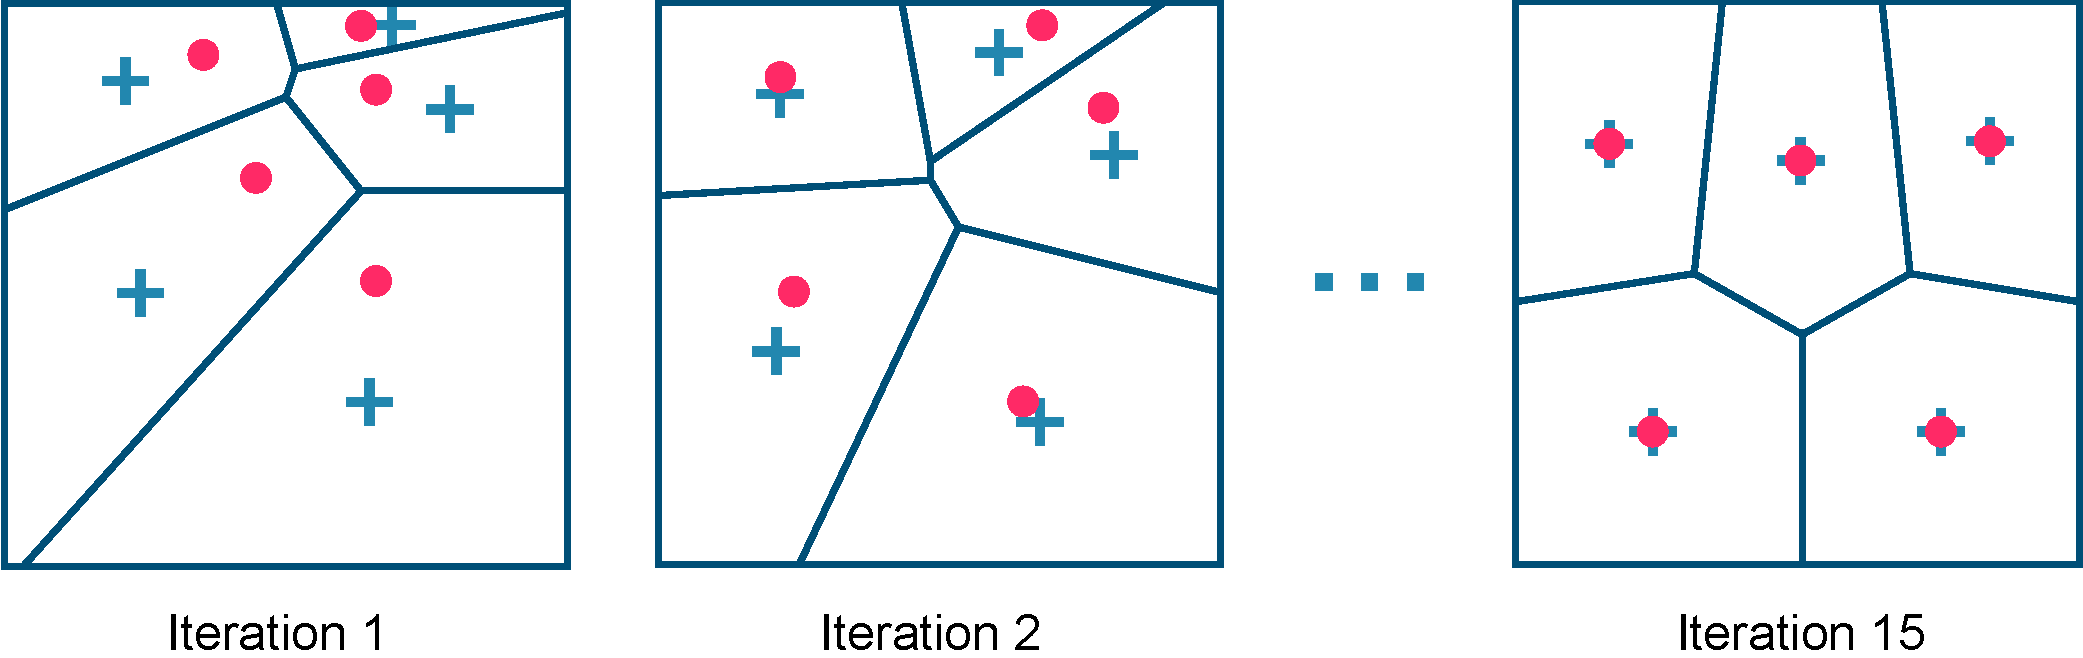
\includegraphics[width=1.0\textwidth]{figures/related/lloyds_method.pdf} 
\caption[An illustration of Lloyd's Method.]
{\label{fig_lloyds_method} 
An illustration of Lloyd's method.
The initial configuration is a Voronoi diagram of point elements (drawn as red dots).
We move the point elements to the centroids of Voronoi cells (drawn as plus signs).
The process is repeated until convergence, producing a Centroidal Voronoi Diagram.
Figure source is Wikipedia, drawn by Dominik Moritz under CC0 1.0.
}
\end{figure}


\begin{figure}
\centering
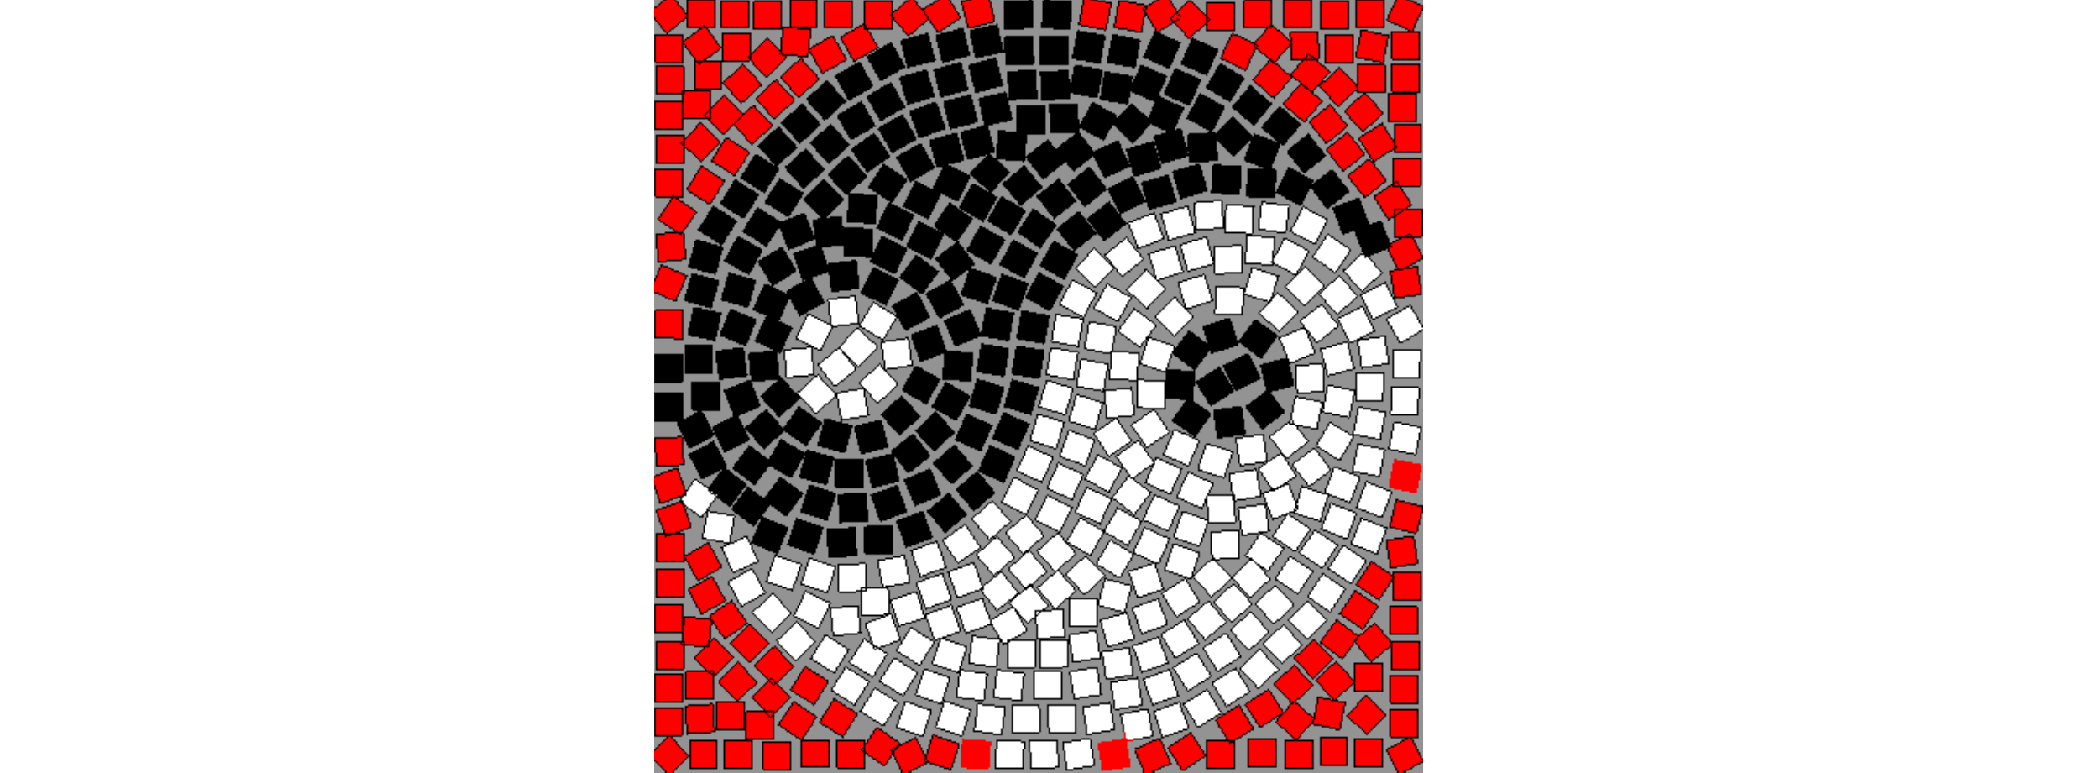
\includegraphics[width=1.0\textwidth]{figures/related/hausner.pdf} 
\caption[Decorative mosaics using Lloyd's method]
{\label{fig_related_hausner} 
Mosaics of square elements generated using Lloyd's method~\cite{Hausner2001}}
\end{figure}


\begin{figure}
\centering
\includegraphics[width=1.0\textwidth]{figures/related/jim_pad.pdf} 
\caption[Examples of packings generated by JIM and PAD]
{\label{fig_related_jim_pad} 
(a) Jigsaw Image Mosaics.
(b) Pyramid of Arclength Descriptor. }
\end{figure}

\begin{figure}
\centering
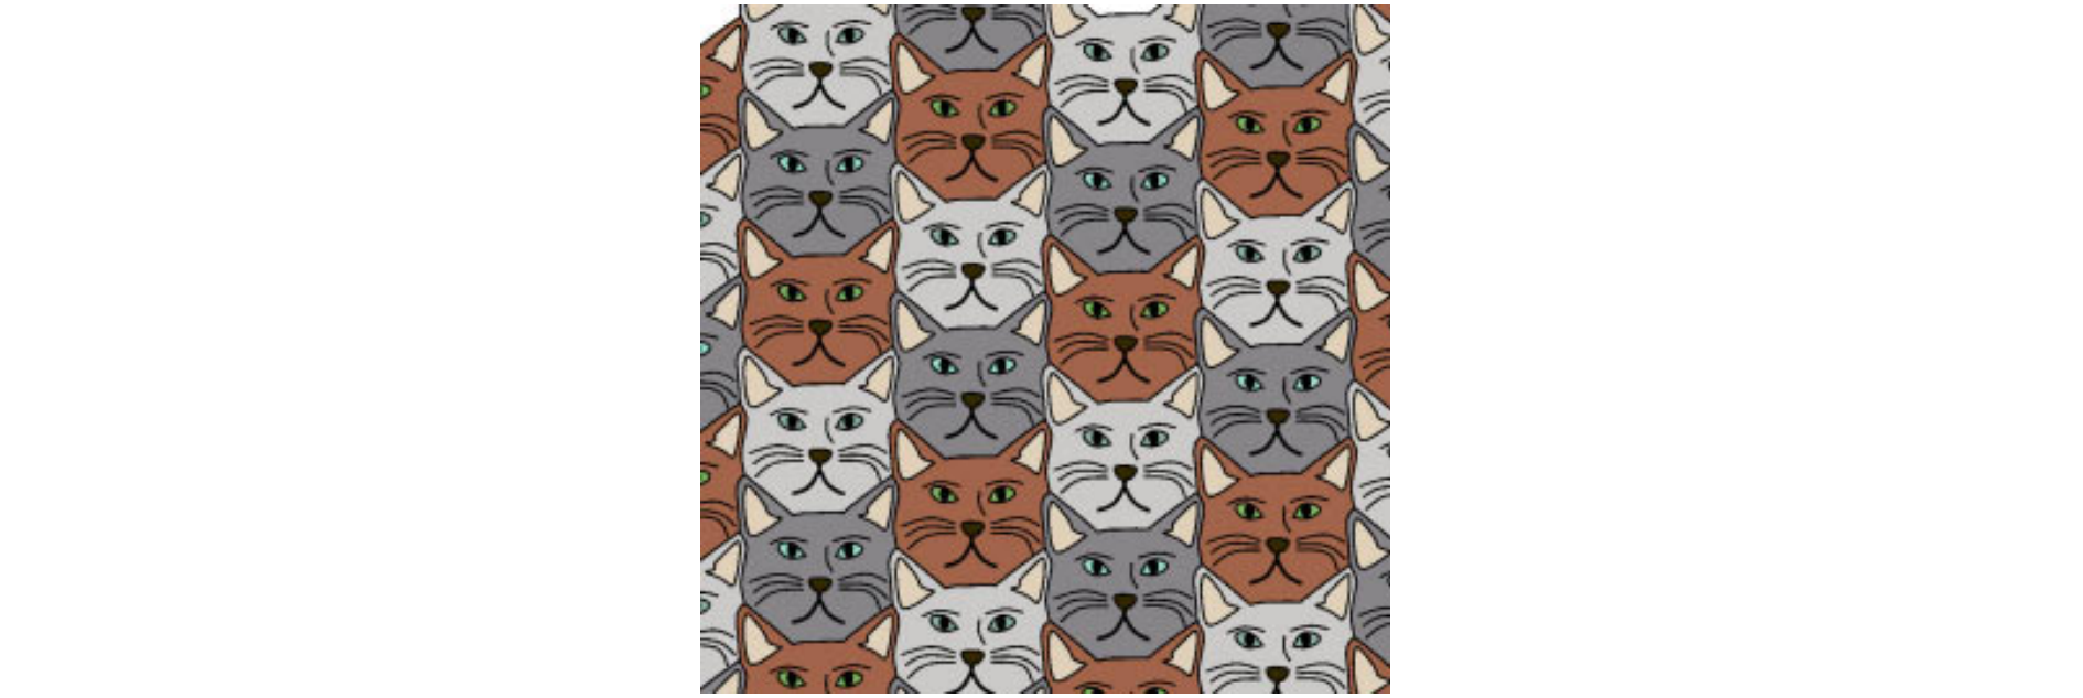
\includegraphics[width=1.0\textwidth]{figures/related/escherization.pdf} 
\caption[An example of a tiling]
{\label{fig_related_escherization} 
A tiling of cats. }
\end{figure}

\begin{figure}
\centering

\includegraphics[width=1.0\textwidth]{figures/related/zehnder.pdf} 
\caption[An example of decorative ornaments filling a surface]
{\label{fig_related_zehnder} 
An example of decorative ornaments filling a surface.}
\end{figure}

\begin{figure}
\centering
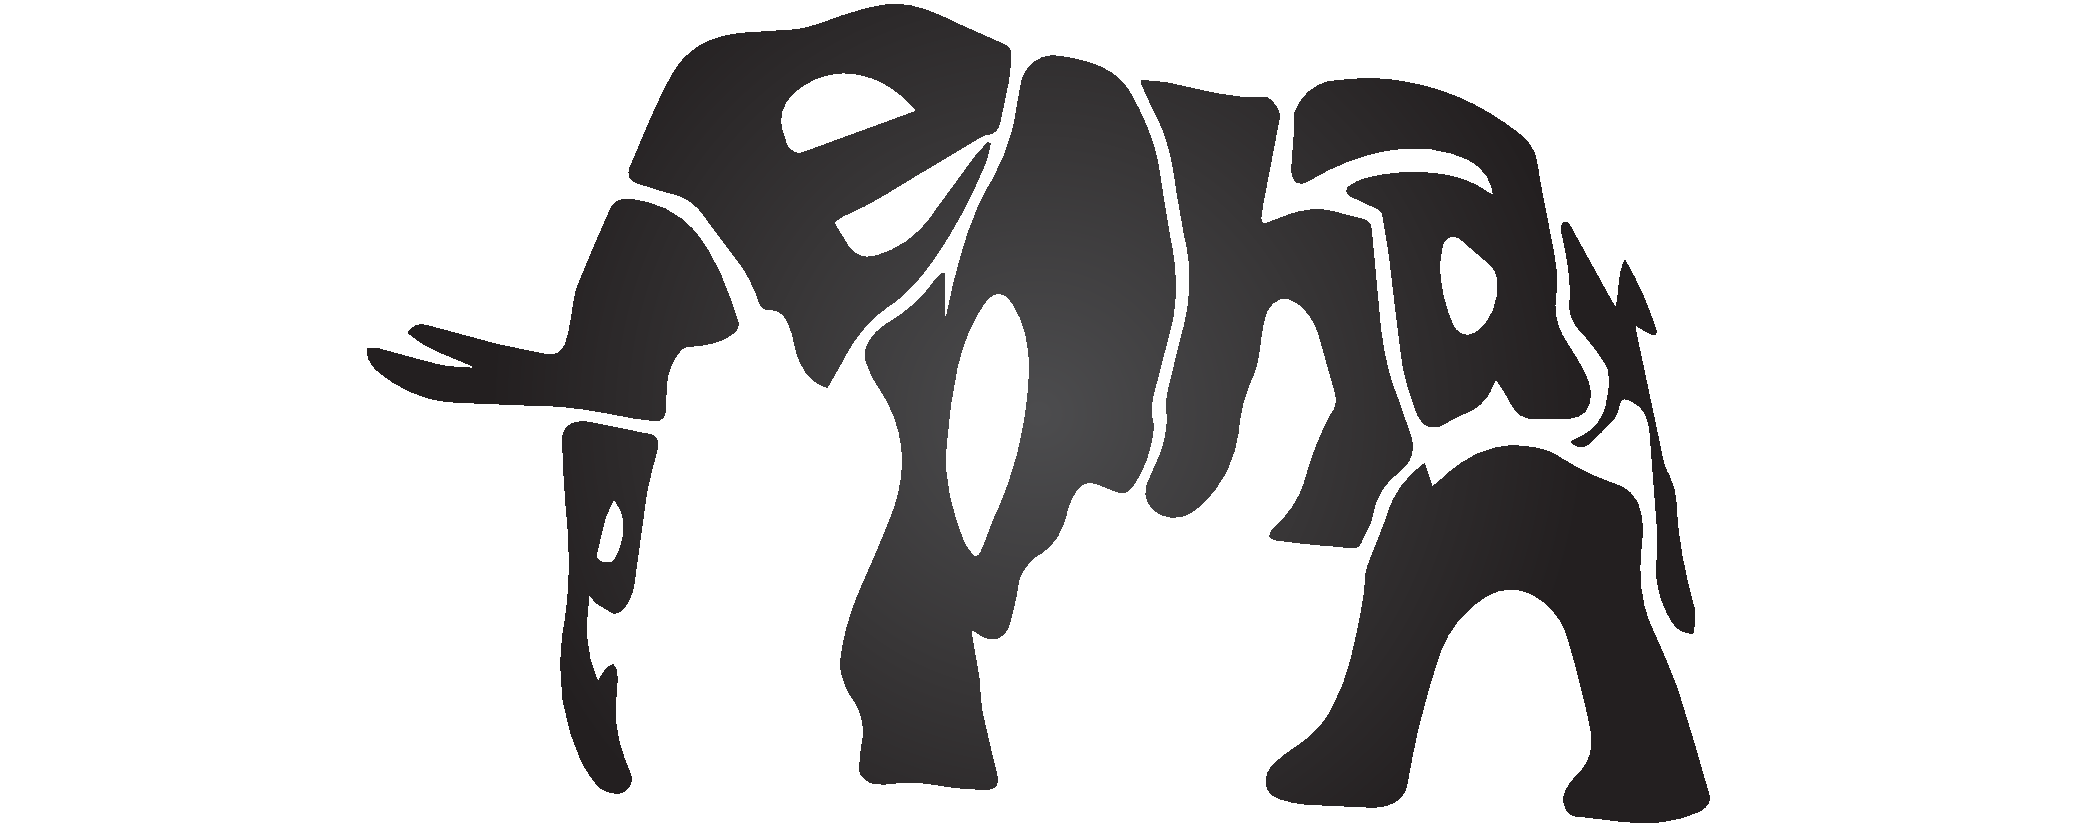
\includegraphics[width=1.0\textwidth]{figures/related/calligraphy.pdf} 
\caption[A calligraphy packing of an ``elephant'']
{\label{fig_calligraphy} 
A calligraphy packing of an ``elephant'.}
\end{figure}


%%%%%%%%%%%%%%%%%%%%%%%%%%%%%%%%%%%%%%%%%%%%%%%%%%%%%%%%%%
\section{2D Packings}
%%%%%%%%%%%%%%%%%%%%%%%%%%%%%%%%%%%%%%%%%%%%%%%%%%%%%%%%%%

%Rigid packing algorithms attempt to distribute elements through rigid transformations.
%These algorithms can be categorized into two groups: iterative methods and data-driven methods.
%Iterative methods start with an initial configuration then they use a variant of Lloyd's method 
%to refine the configuration to an even distribution of elements.
%data-driven methods rely on a shape matching algorithm to find a matching element from
%an element library.
%Some of rigid packing algorithms have an additional step where they 
%correct gaps and overlaps using deformation, the deformation was applied
%locally near edges in a post-processing step after elements
%were frozen in place.

\textbf{Lloyd's method:}
An approach to generate a packing is to start with an initial configuration and iteratively refine it using Lloyd's method
to obtain an even distribution of elements. 
Figure~\ref{fig_lloyds_method} shows an illustration of the original Lloyd's method that can only distribute point elements.
Given an initial distribution of $N$ point elements, 
we first compute a \textit{Voronoi diagram} to partition the plane into $N$ regions such that
all points inside a Voronoi cell are closest to its associated point element.
As an iterative process, 
the Lloyd's method moves every point elements to the centroid of its Voronoi cell, 
then the Voronoi diagram is recomputed.
The process is repeated until the distribution is even.
The final structure is called a \textit{Centroidal Voronoi Diagram} (CVD), 
where all the site points are located at the the centroids of the Voronoi cells. 
Hausner~\cite{Hausner2001} modified the Lloyd's method to distribute square elements into a container 
region, simulating the appearance of traditional mosaics (Figure~\ref{fig_related_hausner}). 
This can be achieved by replacing Euclidean distance with Manhattan distance so that Voronoi cells resemble squares instead of hexagons.
However, Hausner's approach can only move these squares, and a vector field is required to rotate them.
Furthermore, more complicated shapes such as long rectangles would have severe overlaps.
Hiller et al.~\cite{Hiller2003} extended Hausner's idea to generate \textit{Centroidal Area Voronoi Diagram} (CAVD),
a variant of CVD that can accept simple polygonal elements.
This new extension computes main inertia axes for each Voronoi cell so that 
its element can be rotated to get better alignment
with the Voronoi cell boundary.
In a follow up work, Smith et al.~\cite{Smith2005} generated temporally coherent animated mosaics by utilizing CAVD.
Dalal et al.~\cite{Dalal2006} impoved upon CAVD using an FFT-based image correlation to reposition
and rotate elements with their Voronoi cell boundaries, which could be seen as making more effective use of negative
space, and permitting non-convex elements to interlock more than they did in
earlier methods.


%\textbf{Data driven methods:}
\textbf{Data-driven method:} 
A different approach to generate packings is to use a shape matching algorithm
and it requires a library containing a large number of elements.
This is usually done by placing an element one by one until container area is filled.
For each step, a shape matching algorithm selects an 
element that has the best fit with the previously placed elements or the container boundary.
Jigsaw Image Mosaics~\cite{Kim2002} used a geometric hashing to find
a matching element. JIM places elements using a greedy approach, but is able to backtrack 
if previous configuration is more optimal.
Pyramid of Arclength Descriptor~\cite{Kwan2016} developed
a partial shape matching algorithm that can match a subset of element boundary with a portion
of container boundary.

It is also possible to initially partition the container into smaller segments,
then use a shape matching algorithm to independently replace each segment with a matching element.
Huang et al.~\cite{Huang2011} produced Arcimboldo-like collages
by arranging cutout images collected from the internet.
Their container is a larger cutout image which is partitioned into segments
using an image segmentation algorithm.
Each segment is then replaced with a smaller cutout image that has a similar shape and color.

All these data-driven methods require an element library that is big enough,
the more elements in the library will increase their chance to find a compatible element boundary.
However, bigger database means increased computational time.
Collecting a large number of elements is also not always feasible,
for example, if an artist wants to create a packing of a hand-drawn cats,
they may not want to draw 1000 cats which is tedious and repetitive.

%%%%%%%%%%%%%%%%%%%%%%%%%%%%%%%%%%%%%%%%%%%%%%%%%%%%%%%%%%
%\section{Non-rigid Packing Methods}
%%%%%%%%%%%%%%%%%%%%%%%%%%%%%%%%%%%%%%%%%%%%%%%%%%%%%%%%%%

% need to consult to FLOWPAK for variety
\textbf{Deformation-driven method:}
Instead of finding compatible elements,
a deformation-driven method forces elements to create compatibilities and shape variations.
As an advantage, a deformation-driven method can rely on a small size element library.
Peng et al.~\cite{Peng2014} computed layouts by packing and deforming
simple polygons and polyominoes, although their method cannot handle more
complicated shapes, making it unsuitable for our style of packings.
Xu and Kaplan~\cite{Xu2007} and Zou et al.~\cite{Zou2016}
constructed \textit{calligrams} by filling a container with a small
number of deformed letters composing one or two words.  
Their goal was to balance between filling the container and preserving readability.
Abdrashitov et al.~\cite{Abdrashitov2014} developed
a sketch-based interface where an artist can draw curves where square-like elements are placed along it
create a mosaic arrangement.
After the square elements are frozen in place, 
they are deformed to eliminate overlap, to create shape variations, 
and to even even out negative space.  
%Zehnder et al.~\cite{Zehnder2016} proposed an method to
%cover 3D surfaces with deformed ornamental elastic curves.

%Some of rigid packing algorithms have an additional step where they 
%correct gaps and overlaps using deformation, the deformation was applied
%locally near edges in a post-processing step after elements
%were frozen in place.

%%%%%%%%%%%%%%%%%%%%%%%%%%%%%%%%%%%%%%%%%%%%%%%%%%%%%%%%%%
\section{Tilings}
%%%%%%%%%%%%%%%%%%%%%%%%%%%%%%%%%%%%%%%%%%%%%%%%%%%%%%%%%%
\mynote{Need more details on how they work.}
As elements reach perfect compatibility, a packing turns to a tiling.
The element boundaries interlock, leaving no negative space.
Kaplan and Salesin~\cite{Kaplan2000, Kaplan2004} deformed one or two 
input elements into ones that can tile the plane.
Given an input element $E$ they look for a similar tile $T$
from a parameterized tiling space.
Due to high frequency deformations,
$T$ is often perceptually unrecognizable from its silhouette unless an interior picture is added.
They can fail to find $T$ if $E$ has deep concavity, for example, a ``G'' shape.
The tile $T$ also cannot fill a container due to its highly structured boundary.

\mynote{bad...}
Lin et al.~\cite{Lin2018} generated tiling arrangements of two elements that resemble Escher's Sky and Water I.
Each element gradually transition from positive space to negative space. 
The transition directions of both elements are the opposite of each other.



%%%%%%%%%%%%%%%%%%%%%%%%%%%%%%%%%%%%%%%%%%%%%%%%%%%%%%%%%%
\section{Discrete Texture Synthesis}
%%%%%%%%%%%%%%%%%%%%%%%%%%%%%%%%%%%%%%%%%%%%%%%%%%%%%%%%%%
\mynote{Need more details on how they work.}
Some past work has sought to adapt example-based texture synthesis methods
from raster images to vector graphics, producing distributions of rigidly transformed elements
that mimic the statistics of an exemplar.  Barla et al.~\cite{Barla2006} and
Ijiri et al.~\cite{Ijiri2008} use a growth model that copies small neighbourhoods
from the exemplar into a larger output texture.  AlMeraj et al.~\cite{AlMeraj2013}
stamp out copies of the exemplar and discard overlapping elements.
Hurtut et al.~\cite{Hurtut2009} developed a statistical sampling method based
on multitype point processes.  
Loi et al.~\cite{Loi2017} developed a texture synthesis method that
can specify global arrangements, local arrangements, or a blend of multiple arrangements.
These techniques are all concerned with replicating
the uneven element distribution in the exemplar, without regard for negative space.

%%%%%%%%%%%%%%%%%%%%%%%%%%%%%%%%%%%%%%%%%%%%%%%%%%%%%%%%%%
\section{3D Packings}
%%%%%%%%%%%%%%%%%%%%%%%%%%%%%%%%%%%%%%%%%%%%%%%%%%%%%%%%%%
\mynote{Need more details on how they work.}
Gal et al.~\cite{Gal2007B} presented a method for constructing 3D
collages reminiscent of portrait paintings by Arcimboldo.  They
filled a 3D container with overlapping 3D elements using a greedy
approach and a partial shape matching algorithm.
They require a 3D shape database so the method can be considered as data-driven. 
% this one is too narrow, kinda unrelated
Attene~\cite{Attene2015} decomposed a 3D model into parts that pack
tightly into a small build volume, allowing it to 
be 3D printed with less waste material and packed into a smaller box.
Ma et al.~\cite{Ma2018} developed a heuristic method
to create 3D packings that are overlap free.

%%%%%%%%%%%%%%%%%%%%%%%%%%%%%%%%%%%%%%%%%%%%%%%%%%%%%%%%%%
\section{Packings on Surfaces}
%%%%%%%%%%%%%%%%%%%%%%%%%%%%%%%%%%%%%%%%%%%%%%%%%%%%%%%%%%
\mynote{Need more details on how they work.}
\mynote{Chen2016 is also ornamental elastic curves.}
\mynote{Be careful some are overlapping with FLOWPAK.}
Related work in fabrication has sought to cover surfaces with
arrangements of deformed ornamental elements that satisfy manufacturing
constraints such as connectivity.  Chen et al.~\cite{Chen2016}
developed a method to synthesize filigree patterns out of simple elements. 
In later work, Chen et al.~\cite{Chen2017}
generated modular surfaces by computing 
contact point networks of rigid elements.
Zehnder et al.~\cite{Zehnder2016} proposed a deformation-driven method to cover
3D surfaces with ornamental elastic curves.



